%!TEX TS-program = pdflatex
%!TEX root = tesi.tex
%!TEX encoding = UTF-8 Unicode

\chapter{Conclusioni}

\section{Commento Dei Risultati}
Innanzitutto è bisognoso confrontare i risultati ottenuti con gli obbiettivi posti all'inizio di questo documento.
Si ricorda che uno dei principali obbiettivi era quello di non scartare più del 2\% di esemplari Conformi.
Osservando i risultati ottenuti si può vedere che, nonostante il campione a disposizione abbia una numerosità ridotta, nessun Conforme dell'insieme di \textit{test} è stato classificato in modo scorretto.
Questo significa che c'è una quantità di Falsi Positivi pari allo 0\%.
Verificando le capacità del sistema anche sull'insieme d'allenamento, risulta che lo 1.1\% di elementi è stato classificato come Scarto.
Tra questi si trovano principalmente foto scattate ad una distanza superiore alla media.

%Identificare il maggior numero possibile di elementi della classe Scarto, idealmente tutti.
Va fatto notare che difficilmente un sistema è perfetto: infatti di solito richiedere un'alta capacità di riconoscimento per una classe porta ad un calo di accuratezza per un'altra.
%Intuitivamente 
Quindi avere come obbiettivo un sistema che lasci passare tutti i Conformi e allo stesso tempo sia chirurgico nell'identificazione degli Scarti significa porsi di fronte ad una sfida notevole.
L'inseme di algoritmi descritto in questo documento riconosce uno Scarto con un'accuratezza del 93.3\%.
Purtroppo il numero limitato di esemplari per questa classe non ci permette di tracciare delle percentuali che possano definirsi accurate, infatti quel 6.7\% è rappresentato da appena quattro carcasse.
%Dopo aver verificato che queste quattro carcasse presentano colle con caratteristiche simili, non possiamo dire con sicurezza quale sia la frequenza di creazione di quei particolari tipi di colla (di forma molto sottile ed allungata).
Si suppone però che gli esemplari Scarto a nostra disposizione catturino sufficientemente bene la forma più frequente di colla, concludiamo che questo risultato sia soddisfacente.

Inoltre si ritiene necessaria un'ultima considerazione su adattabilità e flessibilità della soluzione proposta.
Entrambi gli algoritmi di \textit{pre} e \textit{post-processing} hanno flessibilità ridotta perché sono stati creati ed impostati manualmente.
È possibile che, al variare della calibratura del processo di raccolta immagini, si ottengano risultati inaspettati.
Basti pensare che le dimensioni della maschera applicata in fase di \textit{pre-processing} non sono adattative, ciò significa che, ad esempio, al variare della distanza della fotocamere dal fondo della carcassa, non si possa esser certi né che tutti i gradini siano visibili, né che le balze vengano nascoste completamente.
Infatti, proprio quest'ultimo è il principale motivo di classificazione errata di alcuni Conformi.
Va però fatto notare che sono algoritmi facilmente modificabili e che la loro calibratura potrebbe essere effettuata durante la calibratura del macchinario, dato che il risultato dipende da pochi parametri.

Per quanto riguarda l'\textit{autoencoder}, il suo allenamento risulta rapido e richiede un numero esiguo di risorse.
In particolar modo non è richiesto che il \textit{dataset} sia etichettato a mano, pratica dispendiosa e prona ad errori.
Inoltre, anche qualora l'inseme di immagini contenesse elementi della classe errata, ciò non sarebbe un problema, perché l'\textit{autoencoder} si adatta agli element più frequenti.
Di conseguenza queste caratteristiche permettono di creare nuovi \textit{dataset} in un tempo molto ridotto rispetto ad altre tecniche.

In conclusione questa soluzione dimostra d'essere valida, permettendo di identificare Conformi e Scarti con una precisione soddisfacente.
Purtroppo le limitazioni dei dati a nostra disposizione non ci permettono di affermare in maniera definitiva che la soluzione, così com'è stata presentata in questo documento, sia pronta per essere utilizzata in applicazioni reali.
Bisogna però dire che questo modello, con le dovute modifiche agli algoritmi di \textit{pre} e \textit{post-processing}, può essere facilmente adattato a problemi di natura simile a quello descritto, grazie alla flessibilità dell'\textit{autoencoder}.


%\section{Soluzione Alternativa}
%È doveroso commentare una promettente soluzione alternativa che riguarda la segmentazione semantica e più nello specifico le U-Net~\cite{unet}.
%La segmentazione semantica permette di associare ad ogni \textit{pixel} di un'immagine una specifica classe.
%Oggi viene usata nei sistemi di guida autonoma, perché permette di identificare e distinguere con precisione la carreggiata, gli eventuali ostacoli, le altre macchine e soprattutto i pedoni e la segnaletica stradale.
%Le reti neurali utilizzate per questo compito vengono chiamate U-Net a causa della loro architettura che, come si vede in figura~\ref{fig:unet}, ricorda la forma di una U.
%Queste reti hanno una struttura simile agli \textit{autoencoder} perché si possono distinguere una fase discendete ed una di risalita, ci sono però due principali differenze:
%\begin{enumerate}
%  \item si vuole mantenere più informazione possibile.
%    Ciò viene effettuato raddoppiando il numero di canali in corrispondenza di ogni \textit{max-pooling layer}.
%
%  \item in corrispondenza dei \textit{layer} con le stesse dimensionalità viene effettuata una copia dei dati dagli strati dell'\textit{encoder} a quelli del \textit{decoder}, ciò permetterà di effettuare una classificazione più precisa.
%
%\end{enumerate}
%Le U-Net vengono allenate per fornire in \textit{output} un'immagine in cui ad aree di \textit{pixel} viene assegnato il colore della classe corrispondente.
%Sia $I$ l'immagine in ingresso e sia $L$ una copia di $I$, in cui ogni elemento è stato colorato a mano con il colore della relativa classe.
%Durante l'allenamento si vuole minimizzare la differenza tra l'immagine $L'$ creata dalla rete e la $L$ fornita.
%In questo modo il modello è spinto a creare delle relazioni tra ciò che è rappresentato nell'immagine in ingresso ed i colori attesi in uscita.
%
%\begin{figure}[ht]
%  \begin{center}
%    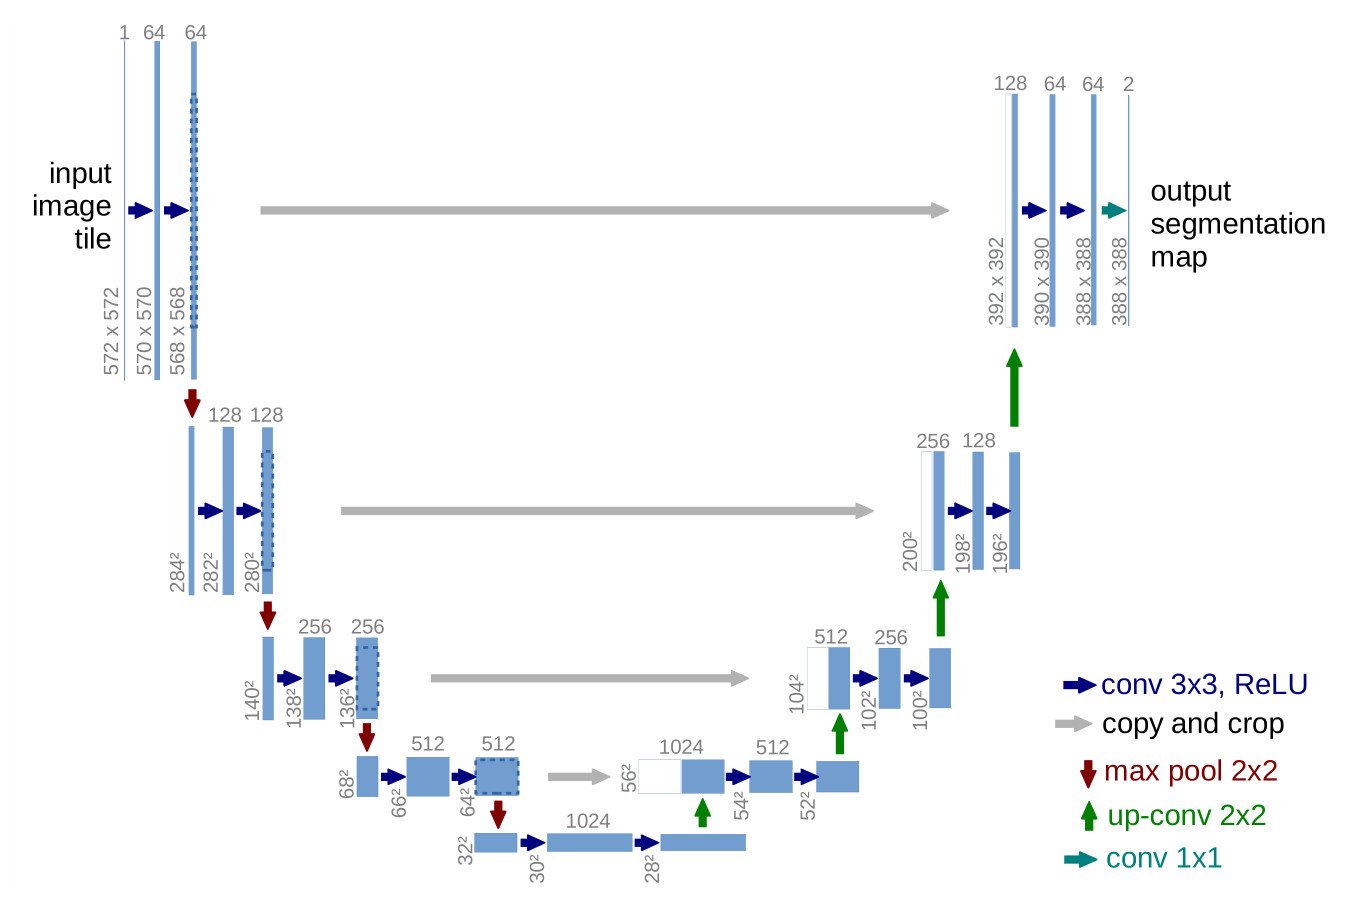
\includegraphics[width=\textwidth]{unet}
%    \caption{Architettura di una U-Net}
%    \label{fig:unet}
%  \end{center}
%\end{figure}
%
%Nel nostro caso il problema della segmentazione, riconosciuto universalmente come un problema di grande complessità, viene semplificato notevolmente: si vuole riconoscere soltanto i \textit{pixel} relativi alla colla.
%Verranno usati solamente due colori, uno sarà associato alla colla, mentre il secondo alla restante parte dell'immagine.
%Il principale problema risiede nel \textit{dataset}.
%Disponendo di solo trenta esemplari risulta difficile, se non impossibile, creare un modello che non sia in forte \textit{overfit} rispetto a quelle specifiche istanze di colla.
%Si è deciso di applicare la tecnica del \textit{data augmentation}, escludendo però alcuni esemplari, utilizzati in un secondo momento per effettuare la validazione del modello.
%Questa tecnica ha permesso di aumentare il numero di esemplari ad un valore superiore a 300, combinando in modo causale tecniche come rotazioni, allungamenti ed accorciamenti, ridimensionamenti e cambi di luminosità.
%Per ogni Scarto è stata creata la rispettiva immagine binaria $L$.
%Ad ogni $L$ sono state applicate le stesse trasformazioni dell'immagine originale, così da generare automaticamente le etichette anche per le immagini create con il \textit{data augmentation}.
%
%Risulta che dopo solo due epoche, la U-Net ha raggiunto un'accuratezza superiore al 95\%, identificando correttamente anche le colle che non le erano mai state sottoposte durante l'allenamento.
%Ciò che più sorprende è la precisione con cui delinea l'area relativa alla colla.
%Per quanto riguarda i Conformi: il modello genera un numero di falsi positivi superiore al 4\%.
%
%Questa tecnica, se si riuscisse a superare l'ostacolo delle dimensioni \textit{dataset}, potrebbe rivelarsi vincente.
%I principali vantaggi rispetto all'utilizzo degli \textit{autoencoder} sono la maggiore flessibilità ed il non dover sviluppare complessi algoritmi di \textit{post-processing}.
%Il principale svantaggio è il dover creare a mano un'immagine per ogni elemento del dataset.
%Questo comporta un grande dispendio di risorse umane sia in fase di creazione delle etichette, ma soprattutto in fase di verifica della correttezza del \textit{dataset}.
%
